\chapter{Solu\c tia propus\u a}

\vspace*{-1cm}
\section{Cerin\c te func\c tionale pentru utilizator \c si \newline nefunc\c tionale}

\subsection{Cerin\c te func\c tionale pentru utilizator}

\begin{itemize}
	\item \textbf{RF-U1} --- \^Inregistrare cont: username, email, telefon, parol\u a; trimitere cod 6 cifre pe email; creare cont dup\u a verificare.
	\item \textbf{RF-U2} --- Autentificare cu email \c si parol\u a; primire token JWT.
	\item \textbf{RF-U3} --- Resetare parol\u a prin email sau telefon (email mascat la c\u autare dup\u a telefon).
	\item \textbf{RF-U4} --- Vizualizare list\u a evenimente viitoare; filtre: nume, jude\c t, dat\u a.
	\item \textbf{RF-U5} --- Pagin\u a detalii eveniment: descriere, imagini, loca\c tie, pre\c t, locuri.
	\item \textbf{RF-U6} --- Cump\u arare bilete nominale (1..N nume); redirect Stripe Checkout.
	\item \textbf{RF-U7} --- Confirmare plat\u a; vizualizare bilete \^in ``Biletele mele'' (viitoare/trecute).
	\item \textbf{RF-U8} --- Editare profil; schimbare parol\u a; \c stergere cont (cu confirmare parol\u a).
\end{itemize}

\subsection{Cerin\c te func\c tionale pentru administrator}

\begin{itemize}
	\item \textbf{RF-A1} --- CRUD evenimente: titlu, descriere, dat\u a, jude\c t, localitate, loca\c tie, pre\c t, locuri, durat\u a, imagini (max 8).
	\item \textbf{RF-A2} --- List\u a participan\c ti per eveniment; check-in.
	\item \textbf{RF-A3} --- Promovare/revocare rol admin (cu parol\u a autorizare); protec\c tie ultim admin.
\end{itemize}

\subsection{Cerin\c te nefunc\c tionale}

\begin{itemize}
	\item \textbf{RNF-1 Securitate} --- bcrypt, JWT, hash token-uri/coduri, CORS, rate limiting.
	\item \textbf{RNF-2 Disponibilitate} --- API stateless; DB rela\c tional\u a.
	\item \textbf{RNF-3 UX} --- Responsive; tem\u a dark; mesaje eroare clare.
	\item \textbf{RNF-4 Mentenabilitate} --- Separare frontend/backend; migr\u ari SQL.
	\item \textbf{RNF-5 Portabilitate} --- Node.js 18+, PostgreSQL 14+.
\end{itemize}

\section{Arhitectura sistemului}

ManFast urmeaz\u a arhitectura \textbf{client-server} \^in trei straturi:

\begin{enumerate}
	\item \textbf{Strat prezentare} --- SPA React (Vite), routing React Router, context autentificare, apeluri \texttt{fetch} c\u atre API.
	\item \textbf{Strat aplica\c tie} --- Express: rute \texttt{/api/auth}, \texttt{/api/events}, \texttt{/api/tickets}; middleware JWT \c si \texttt{requireAdmin}.
	\item \textbf{Strat date} --- PostgreSQL; fi\c siere statice imagini \^in \texttt{uploads/}.
\end{enumerate}

Servicii externe: \textbf{Stripe} (pl\u a\c ti), \textbf{Brevo SMTP} (email verificare \c si reset).


\begin{figure}[htbp]
	\centering
	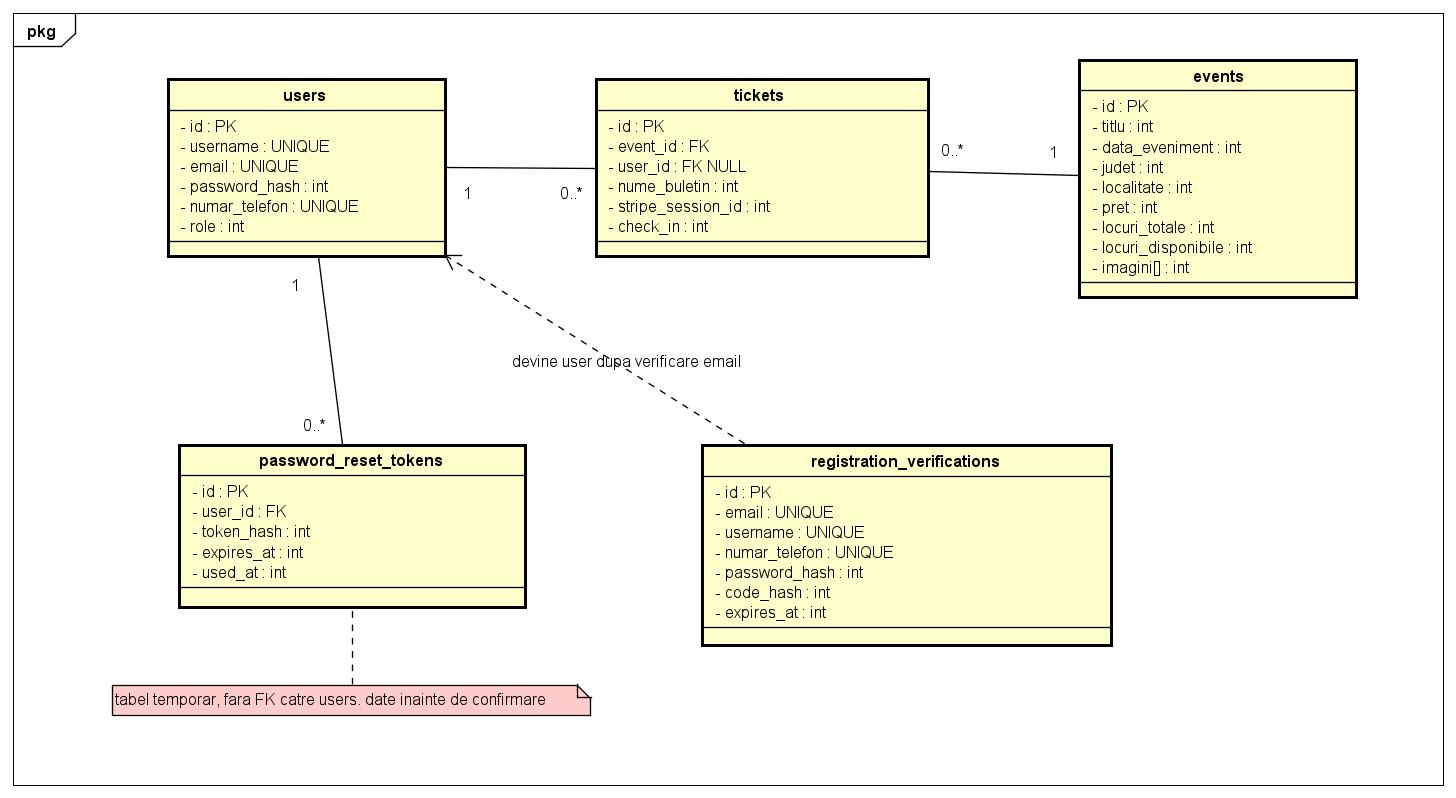
\includegraphics[width=1\textwidth]{Model de domeniu _ ERD ManFast.jpg}
	\caption{Arhitectura sistemului ManFast}
	\label{fig:l2f1}
\end{figure}

Instruc\c tiuni inserare: Diagrama blocuri: Browser (React+MUI) -> HTTPS/JSON -> Express API -> PostgreSQL; lateral Stripe \c si Brevo SMTP. Tool: draw.io, Lucidchart sau PowerPoint. Export PNG 300dpi, l\u a\c time ~14cm \^in document.


\section{Tehnologii utilizate}

\begin{table}[htbp]
	\centering
	\begin{tabular}{|l|p{8cm}|}
		\hline
		\textbf{Tehnologie} & \textbf{Rol} \\
		\hline
		React 19 + Vite 8 & Frontend SPA, HMR dev \\
		\hline
		Material UI 9 & Componente UI, tem\u a dark \\
		\hline
		Express 4 & API REST, Multer upload \\
		\hline
		PostgreSQL & Persisten\c t\u a rela\c tional\u a \\
		\hline
		JWT + bcrypt & Auth \c si hash parole \\
		\hline
		Stripe Checkout & Pl\u a\c ti card RON \\
		\hline
		Nodemailer + Brevo & Email SMTP \\
		\hline
	\end{tabular}
	\caption{Stack tehnologic ManFast}
	\label{tab:tech}
\end{table}

React [8] gestioneaz\u a starea UI \c si re-renderarea eficient\u a. Vite ofer\u a build rapid. Express [11] ruteaz\u a cererile HTTP. pg conecteaz\u a la PostgreSQL. Stripe SDK creeaz\u a sesiuni Checkout.

\section{Diagrame UML}
\subsection{Cazuri de utilizare}

Actorii principali sunt Utilizatorul (autentificat sau nu) \c si Administratorul. Utilizatorul
poate \^inregistra cont, autentifica, filtra evenimente, cump\u ara bilete, gestiona profilul. Administratorul public\u a evenimente, face check-in, gestioneaz\u a al\c ti admini. 

\begin{figure}[htbp]
	\centering
	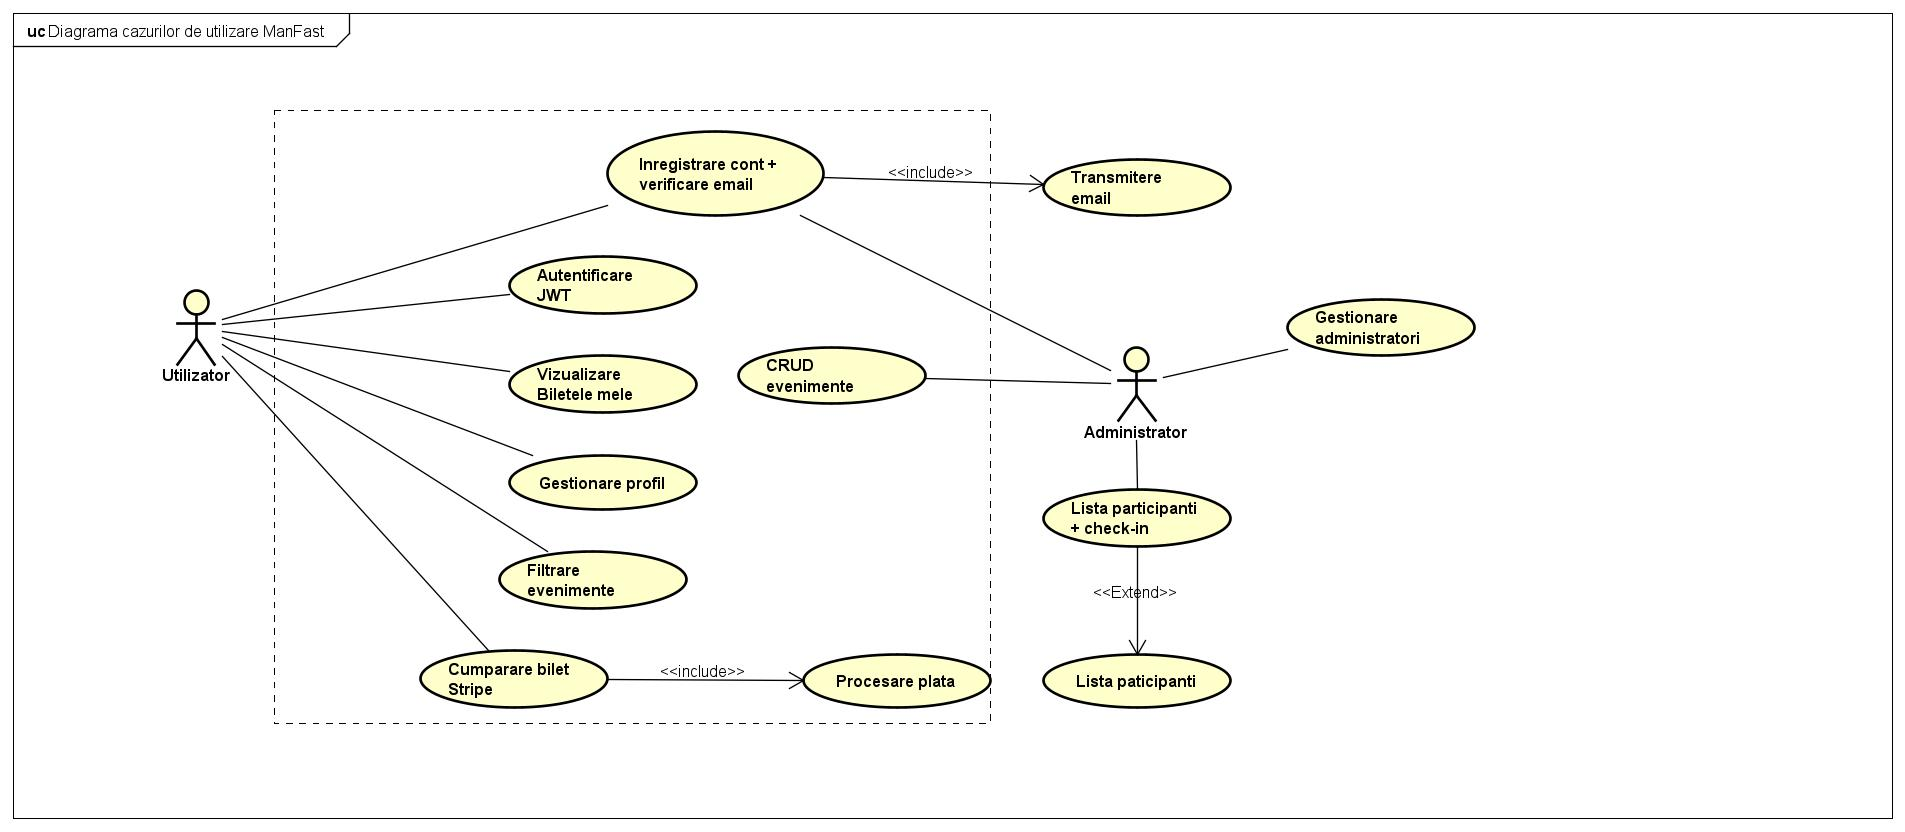
\includegraphics[width=1\textwidth]{Diagrama cazurilor de utilizare ManFast.jpg}
	\caption{ Diagrama cazurilor de utilizare}
	\label{fig:l2f1}
\end{figure}

Instruc\c tiuni inserare: UML use case: actor Utilizator (register, login, filtre, cump\u ar\u a bilet, profil); actor Admin (CRUD eveniment, check-in, promovare admin). Tool: StarUML, draw.io. Include sistem boundary ``ManFast''.

\subsection{Secven\c ta de \^inregistrare cu verificare prin email}

Flux: Frontend POST /register-> Backend valideaz\u a, salveaz\u a \^in \linebreak \texttt{registration\_verifications},
trimite cod SMTP -> Frontend POST /register/verify -> INSERT \texttt{users}.

\begin{figure}[htbp]
	\centering
	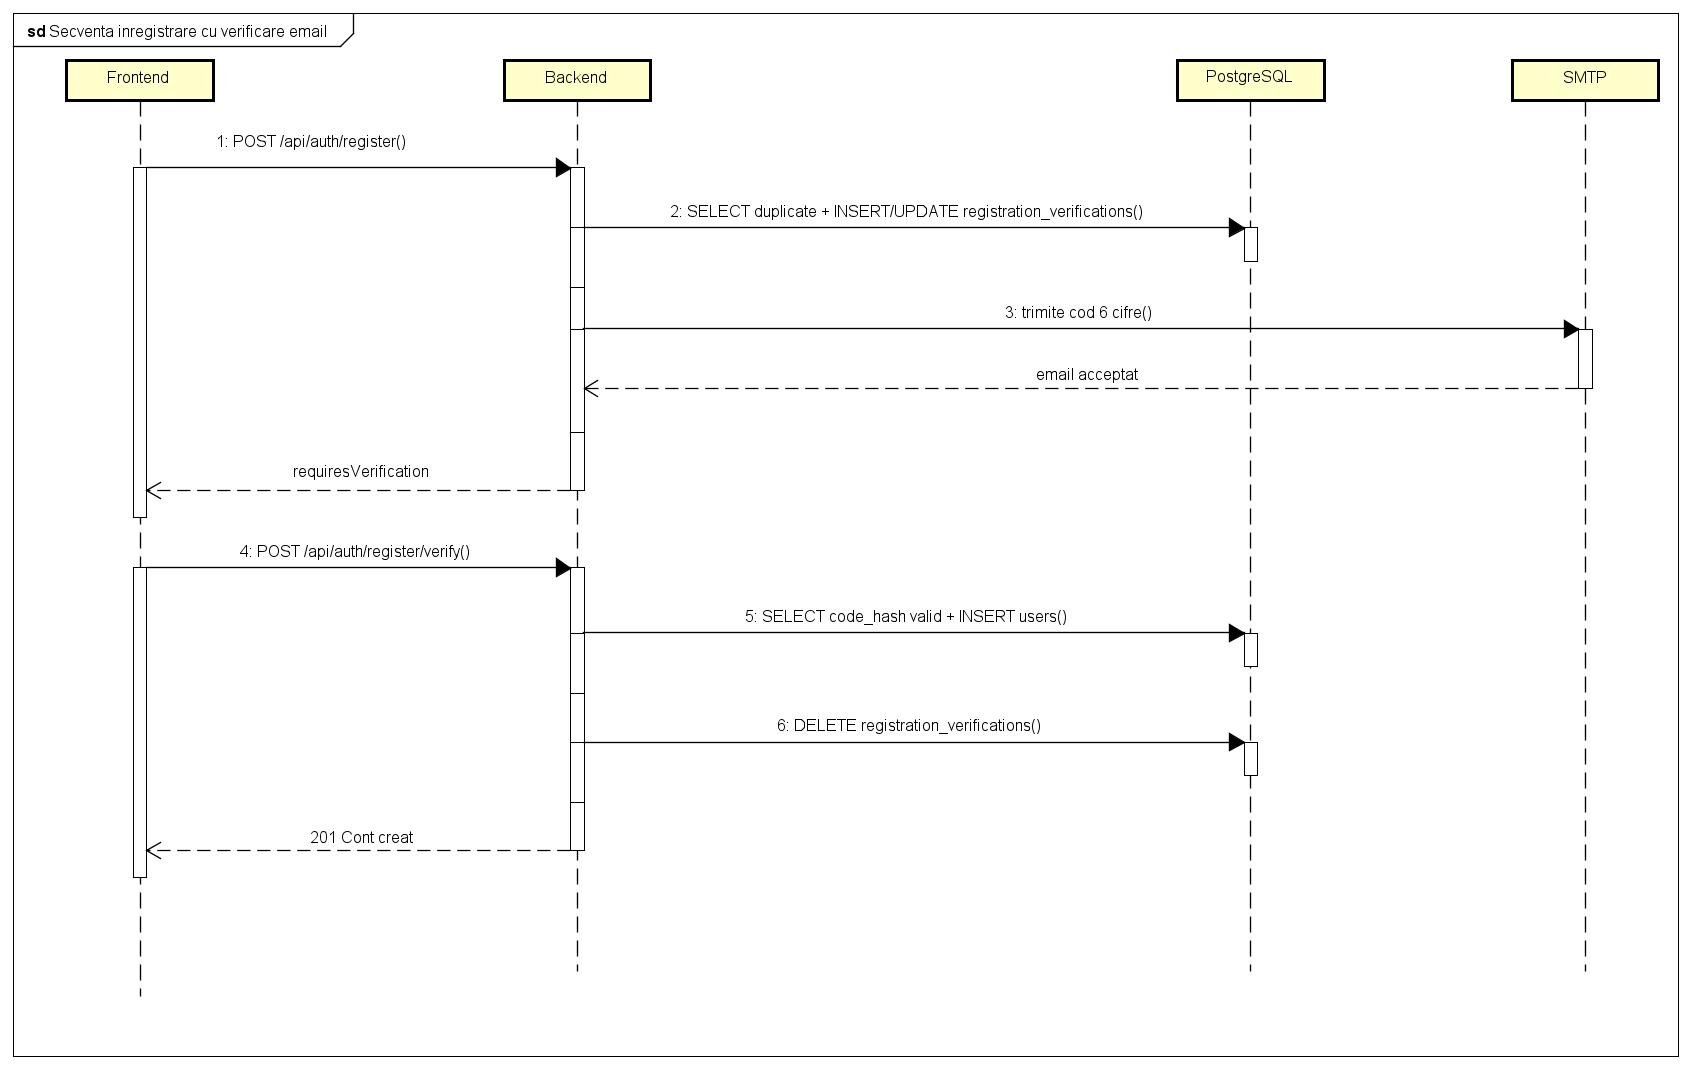
\includegraphics[width=1\textwidth]{Secventa inregistrare cu verificare email.jpg}
	\caption{Diagrama de secven\c t\u a - \^inregistrarea cu email}
	\label{fig:l2f1}
\end{figure}

Instruc\c tiuni inserare: Participan\c ti: Utilizator, Frontend, Backend, PostgreSQL, SMTP. Mesaje:
register, salveaz\u a temp, trimite cod, verify, creare user. Nota\c tii pe fiecare s\u ageat\u a.

\subsection{Secven\c ta pentru plata prin Stripe}

Flux: Frontend POST create-checkout-session -> redirect Stripe -> success URL -> confirm-payment -> INSERT tickets, UPDATE locuri.

Instruc\c tiuni inserare: Participan\c ti: Utilizator, Frontend, Backend, Stripe, DB. Include metadata session \c si confirm-payment.

\begin{figure}[htbp]
	\centering
	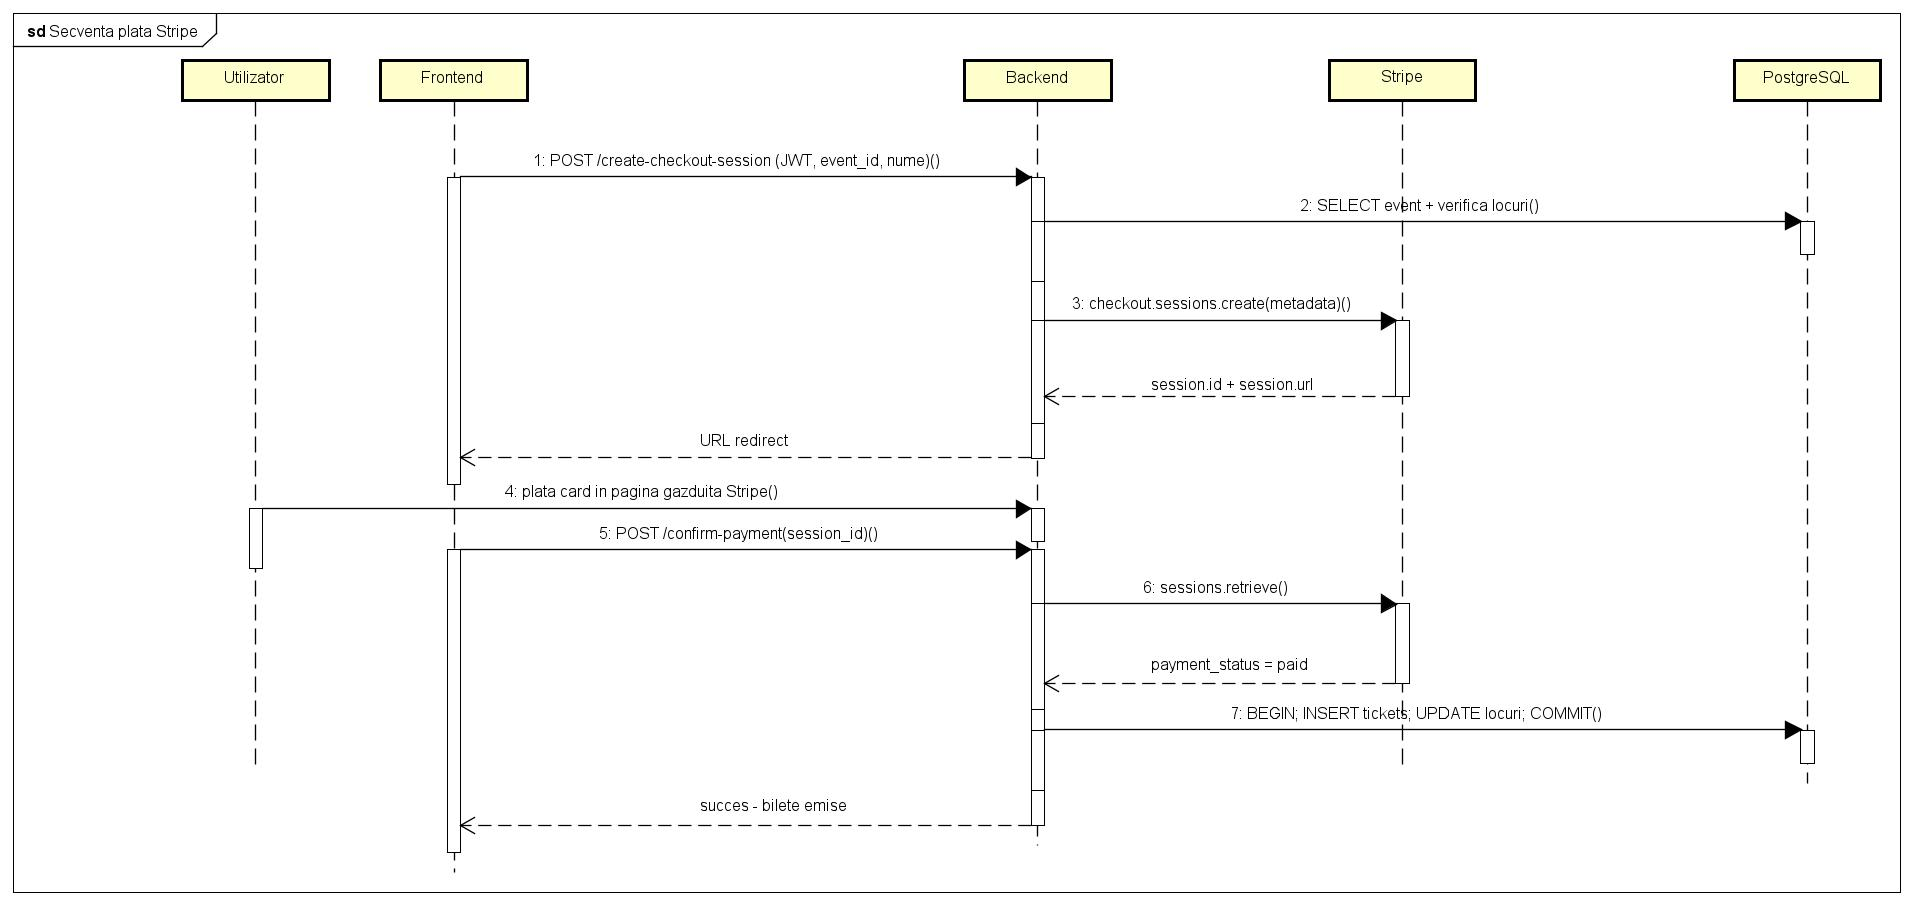
\includegraphics[width=1\textwidth]{Secventa plata Stripe.jpg}
	\caption{Diagrama de secven\c t\u a - plata Stripe}
	\label{fig:l2f1}
\end{figure}


\subsection{Activitatea la check-in \c si admin}

Instruc\c tiuni inserare: Flowchart: admin selecteaz\u a eveniment -> list\u a participan\c ti -> validare bilet -> UPDATE check\_in=true sau mesaj eroare

\begin{figure}[htbp]
	\centering
	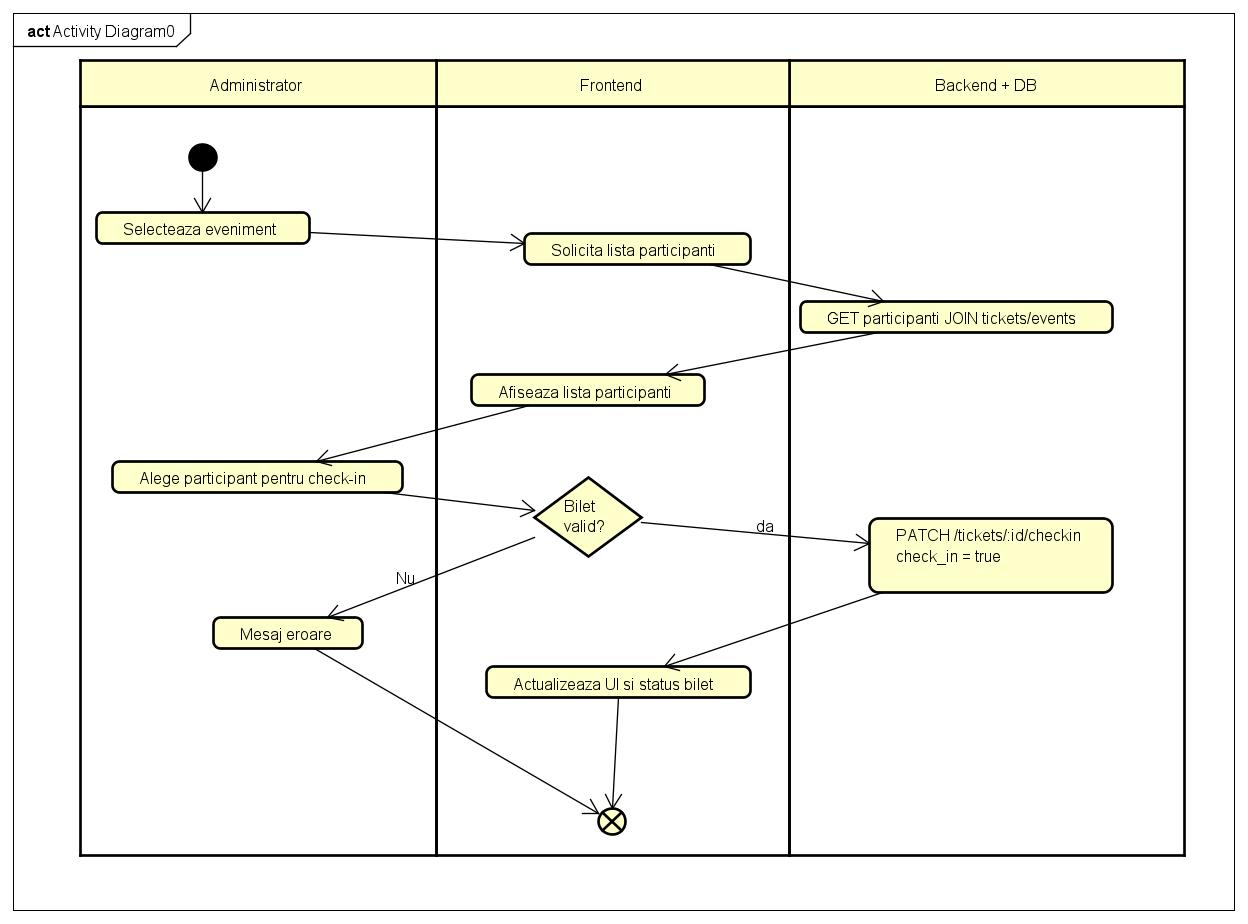
\includegraphics[width=1\textwidth]{Activity Diagram0.jpg}
	\caption{Diagrama de activitate - check-in}
	\label{fig:l2f1}
\end{figure}

\subsection{Proiectarea bazei de date}

Tabele principale: \texttt{users, events, tickets, password\_reset\_tokens, \linebreak registration\_verifications}

Rela\c tii: \texttt{events} 1:N \texttt{tickets; users} 1:N \texttt{tickets} (ON DELETE SET NULL); \texttt{users} 1:N token-uri reset; verific\u ari \^inregistrare temporare p\^an\u a la confirmare. 

\begin{figure}[htbp]
	\centering
	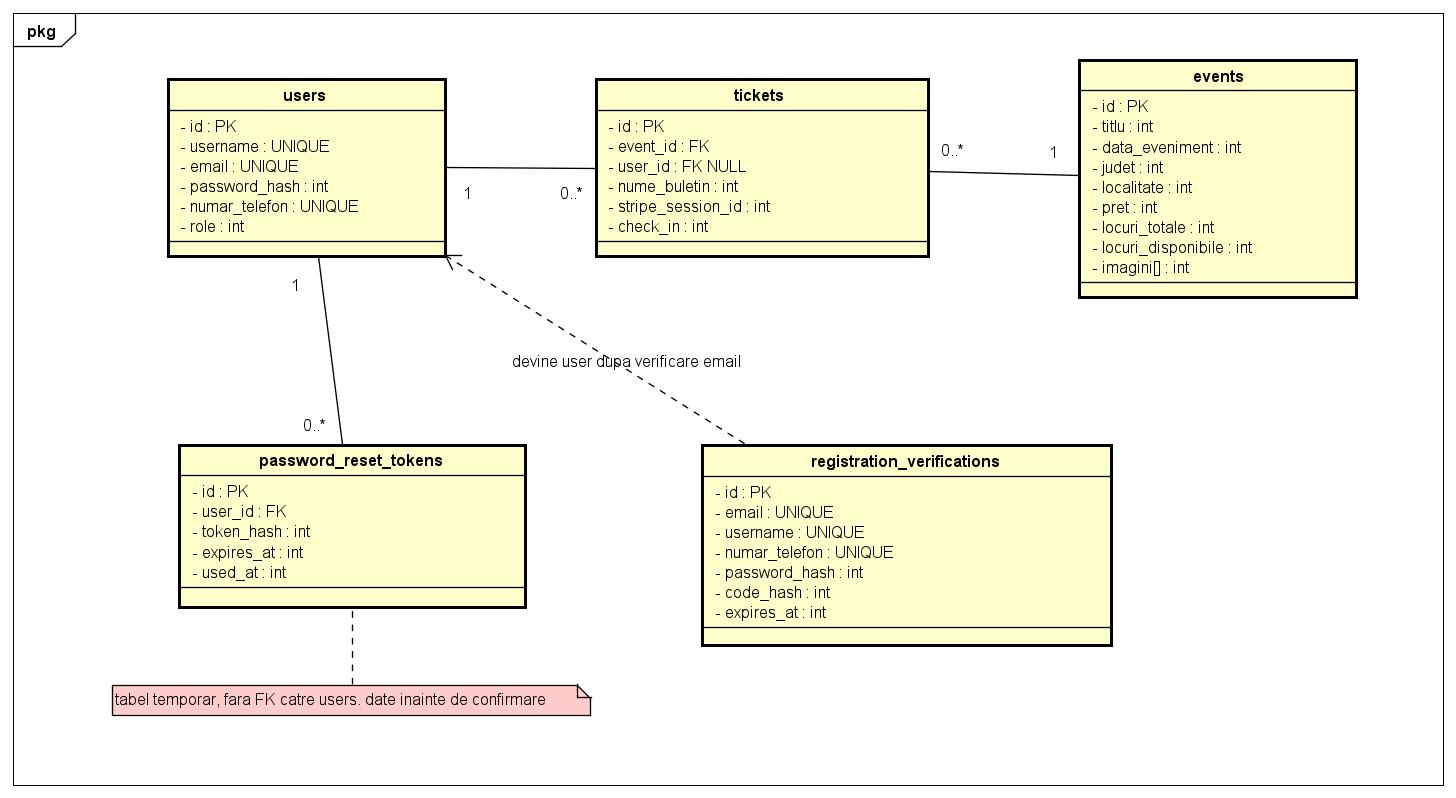
\includegraphics[width=1\textwidth]{Model de domeniu _ ERD ManFast.jpg}
	\caption{Diagrama entitate- rela\c tie}
	\label{fig:l2f1}
\end{figure}


\section{Proiectarea bazei de date}





Tabele principale: \texttt{user, events, tickets, password\_reset\_token, \linebreak registration\_verifi}

Rela\c tii: \texttt{events} 1:N \texttt{tickets; user} 1:N \texttt{tickets} (ON DELETE SET NULL) \texttt{user} 1:N token-uri reset \c si verific\u ari \^inregistrare temporare p\^an\u a la confirmare.




\section{Implementarea func\c tionalit\u a\c tilor cheie}
\subsection{Autentificarea \c si verificarea prin email}

Generarea codului \c si a hash-ului

\begin{lstlisting} 
	function genereazaCodVerificare() {
		return String(crypto.randomInt(100000, 1000000));
	}
	function hashCodVerificare(cod) {
		return crypto.createHash('sha256')
		.update(String(cod).trim()).digest('hex');
	}
\end{lstlisting}

La \texttt{POST /register/verify}, codul este comparat cu \texttt{code\_hash}, expirarea verificat\u a, apoi utilizatorul inserat \^in \texttt{users}. Login-ul genereaz\u a JWT: 

\begin{lstlisting}
	const token = jwt.sign(
	{ id: user.id, role: user.role },
	process.env.JWT_SECRET,
	{ expiresIn: '24h' }
	);
\end{lstlisting}

\subsection{Pl\u a\c ti prin Scripe}

Crearea sesiunii Checkout (extras):

\begin{lstlisting}
	const session = await stripe.checkout.sessions.create({
		payment_method_types: ['card'],
		line_items: [{ 
			price_data: {
				currency: 'ron',
				product_data: { name: `Bilet - ${event.titlu}` },
				unit_amount: Math.round(Number(event.pret) * 100),
			}, 
			quantity: cantitate 
		}],
		mode: 'payment',
		success_url: `${frontendUrl}/payment-success?session_id={CHECKOUT_SESSION_ID}`,
		metadata: { 
			event_id, 
			user_id, 
			nume_participanti: JSON.stringify(nume)
		}
	});
\end{lstlisting}

\texttt{confirm-payment} verific\u a \texttt{session.payment\_status} === '\texttt{paid}', insereaz\u a
c\^ate un r\^and \texttt{tickets} per nume \c si decrementeaz\u a \texttt{locuri\_disponibile} \^intr-o tranzac\c tie.

\subsection{Gestionare evenimente}

Crearea evenimentului folose\c ste Multer pentru imagini \c si validare jude\c t din lista fix\u a (42 jude\c te). La INSERT, \texttt{locuri\_disponibile = locuri totale}. Editarea permite ad\u augare incremental\u a de imagini. \c Stergerea elimin\u a evenimentul \c si biletele asociate (CASCADE)

\subsection{Frontend}

\texttt{AuthContext} stocheaz\u a \texttt{user} \c si \texttt{token} \^in \texttt{localStorage}. \texttt{apiFetch} \linebreak ata\c seaz\u aheader Authorization. Rute protejate: \texttt{/profile, /my-tickets, /admin} (AdminRoute).



\section{Securitate}

\begin{itemize}
	\item Parole: bcrypt cost 10; niciodat\u a \^in clar \^in DB.
	\item JWT: secret separat de Stripe; expirare 24h.
	\item Coduri email \c si token reset: SHA-256 \^in DB.
	\item Rate limit: max 3 coduri / 15 min (produc\c tie); cooldown 60s retrimitere.
	\item CORS: doar \texttt{FRONTEND\_URL}.
	\item Admin: ultimul admin protejat la \c stergere/revocare.
	\item \c Stergere cont: confirmare parol\u a obligatorie.
\end{itemize}

Implementarea respect\u a recomand\u arile OWASP [3] pentru autentificare \c si gestionarea sesiunilor \^in contextul unei aplica\c tii web educa\c tionale/prototip production-ready.

\section{Scenarii de utilizare pe tipuri de evenimente}

Aceast\u a sec\c tiune descrie modul \^in care acelea\c si func\c tionalit\u a\c ti ale platformei sunt valorificate \^in scenarii reprezentative. Scopul este de a demonstra flexibilitatea modelului simplu eveniment--bilet, f\u ar\u a a impune module separate per domeniu.

\subsection{Scenariul 1: Conferin\c t\u a universitar\u a}

Context: Facultatea organizeaz\u a o conferin\c t\u a \c stiin\c tific\u a cu 150 de locuri, taxa de participare 120 RON, desf\u a\c surare \^in Constan\c ta.

\hspace*{2ex} \textbf{Pa\c si organizator:}
\begin{enumerate}
	\item Administratorul creeaz\u a evenimentul: titlu, descriere (program, speakeri), dat\u a, jude\c t Constan\c ta, localitate, loca\c tie (sal\u a), pre\c t 120, locuri 150, durat\u a 8 ore, imagini (banner conferin\c t\u a).
	\item Public\u a link-ul c\u atre pagina principal\u a; participan\c tii filtreaz\u a dup\u a dat\u a sau jude\c t.
	\item Monitorizeaz\u a \texttt{locuri\_disponibile} \c si lista participan\c tilor.
	\item La intrare, efectueaz\u a check-in pe baza numelui de pe bilet.
\end{enumerate}

\textbf{Pa\c si organizator:} Pa\c si participant: \^inregistrare cont, verificare email, cump\u arare bilet nominal, prezentare la recep\c tie. Biletul din ``Biletele mele'' confirm\u a plata \c si identitatea.

\subsection{Scenariul 2 \^in care concertul este \^in aer liber}

\textbf{Context:} Asocia\c tie cultural\u a organizeaz\u a un concert local, 500 locrui, bilet 50 RON, galerie foto arti\c sti.

\textbf{Particularit\u a\c ti:} Galeria cu multiple imagini spore\c ste atractivitatea paginii de detalii. Filtrarea pe jude\c t ajut\u a publicul din zon\u a. V\^anzarea poate include mai multe bilete \^intr-o singur\u a tranzac\c tie Stripe (familie, grup de prieteni), fiecare nume completat corespunde unui bilet nominal.

\textbf{Limit\u ari actuale:} Nu exist\u a categorii de pre\c t (VIP, standard) sau hart\u a locurilor --- extensii posibile prin ad\u augarea unui c\^amp \texttt{tip\_bilet} \^in schema bazei de date.

\subsection{Scenariul 3: Meeting corporate / training}

\textbf{Context:} Firma de IT organizeaz\u a un workshop de o zi, 30 locuri, participare gratuit\u a sau cu pre\c t simbolic

Context: Club sportiv local, turneu cu taxa de \^inscriere, necesitate nume conform buletinului.
{Utilizare:} Chiar \c si la pre\c t mic, Stripe permite monetizare. Alternativ, organizatorul poate
seta pre\c t 1 RON pentru testare. Check-in-ul din admin ofer\u a lista de prezen\c t\u a pentru raport intern. Verificarea email la \^inregistrare reduce \^inscrierile fictive.

\subsection{Scenariul 4: Competi\c tie sportiv\u a amatorial\u a}

\textbf{Context:} Club sportiv local, turneu cu taxa de \^inscriere, necesitate nume conform buletinului.

\textbf{Utilizare:} C\^ampul \texttt{nume} buletin la cump\u arare capteaz\u a numele participantului. Check-in manual valideaz\u a prezen\c ta. Aceast\u a ni\c s\u a folose\c ste acelea\c si mecanisme ca conferin\c ta, f\u ar\u a tabele suplimentare pentru echipe sau clasamente. 

\subsection{Matricea func\c tionalit\u a\c tilor \c si scenarii}

\begin{table}[htbp]
	\centering
	\begin{tabular}{|l|c|c|c|c|}
		\hline
		\textbf{Func\c tionalitate} & \textbf{Conf.} & \textbf{Concert} & \textbf{Meeting} & \textbf{Sport} \\ \hline
		Filtrare jude\c t/dat\u a & Da & Da & Da & Da \\ \hline
		Galerie imagini & Da & Da & Op\c tional & Op\c tional \\ \hline
		Plat\u a Stripe RON & Da & Da & Da & Da \\ \hline
		Bilete multiple / tranzac\c tie & Da & Da & Rar & Da (echipe mici) \\ \hline
		Check-in admin & Da & Da & Da & Da \\ \hline
		Nume nominal (buletin) & Op\c tional & Op\c tional & Op\c tional & Da \\ \hline
	\end{tabular}
	\caption{Func\c tionalit\u a\c ti utilizate \^in scenarii}
	\label{tab:functionalitati_scenarii}
\end{table}

\subsection{Modelul unificat de date}

Decizia de a nu specializa tabelele per tip de eveniment (conferin\c t\u a vs. concert) simplific\u a mentenan\c ta \c si permite unui singur panou admin s\u a gestioneze toate formatele. C\^ampurile \texttt{titlu, descriere, data eveniment, judet, pret, locuri totale \linebreak si imagini} sunt suficient de generice; semantica (``taxa conferin\c t\u a'' vs. ``bilet concert'') este pur textual\u a, definit\u a de organizator.

Aceste scenarii pot fi reproducte \^in cadrul demonstra\c tiei aplica\c tiei \c si documentate prin capturi de ecran \^in capitolul 4.

\section{Fragmente suplimentare de implementare}
\subsection{Rate limiting la \^inregistrare}

Func\c tia depasesteLimitaCoduri limiteaz\u a abuzul de retrimitere cod email \^in produc\c tie:

\begin{lstlisting}
	function depasesteLimitaCoduri(row) {
		if (isDev) return null;
		
		const secundeDeLaUltimulCod =
		(Date.now() - new Date(row.last_code_sent_at).getTime()) / 1000;
		
		if (secundeDeLaUltimulCod < COOLDOWN_RETRIMITERE_SEC) {
			return { status: 429, error: 'Asteapta inainte de un cod nou.' };
		}
		
		if (inFereastraDe15Minute(row.last_code_sent_at)
		&& row.codes_sent >= MAX_CERERI_COD_15_MIN) {
			return { status: 429, error: 'Prea multe cereri de cod.' };
		}
		
		return null;
	}
\end{lstlisting}

\^In modul development (\texttt{NODE\_ENV} diferit de '\texttt{production}'), limitarea este dezactivat\u a pentru a facilita testarea repetat\u a a fluxului de \^inregistrare f\u ar\u a a a\c stepta cooldown-ul de 60 de secunde

\subsection{Middleware autentificare JWT}

Middleware-ul \texttt{authenticateToken} extrage token-ul din header \texttt{Authorization}: \texttt{Bearer}, verific\u a semn\u atura cu JWT\_SECRET \c si ata\c seaz\u a req.user pentru rutele protejate:

\begin{lstlisting}
	function authenticateToken(req, res, next) {
		const authHeader = req.headers['authorization'];
		const token = authHeader && authHeader.split(' ')[1];
		
		if (!token) return res.status(401).json({ error: 'Token lipsa' });
		
		jwt.verify(token, process.env.JWT_SECRET, (err, user) => {
			if (err) return res.status(403).json({ error: 'Token invalid' });
			req.user = user;
			next();
		});
	}
\end{lstlisting}

\texttt{requireAdmin} verific\u a suplimentar \texttt{req.user.role === 'admin'}, return\^and 403 pentru utilizatori obi\c snui\c ti. Aceast\u a separare permite reutilizarea autentific\u arii pe rute mixte (ex. /auth/me vs. /events POST).

\subsection{Validare evenimente la creare}

La \texttt{POST /events}, backend-ul valideaz\u a jude\c tul din lista fix\u a, pre\c tul pozitiv, locuri disponibile \c si proceseaz\u a upload-ul Multer:

\begin{lstlisting}
	const JUDETE_VALIDE = ['Alba', 'Arad', ..., 'Vaslui', 'Vrancea'];
	
	if (!JUDETE_VALIDE.includes(judet)) {
		return res.status(400).json({ error: 'Judet invalid' });
	}
	
	const locuriTotale = parseInt(locuri_totale, 10);
	
	if (isNaN(locuriTotale) || locuriTotale < 1) {
		return res.status(400).json({ error: 'Locuri invalide' });
	}
\end{lstlisting}

Imaginile sunt salvate \^in \texttt{uploads/events/} cu nume unic (timestamp + random), iar URL-urile relative sunt stocate \^in coloana \texttt{imagini} de tip \texttt{TEXT[]}.

\subsection{Componenta AdminRoute (frontend)}
Ruta \texttt{/admin} este protejat\u a pe client prin verificarea rouluiu din contex:

\begin{lstlisting}
	function AdminRoute({ children }) {
		const { user, loading } = useAuth();
		
		if (loading) return <CircularProgress />;
		
		if (!user || user.role !== 'admin') {
			return <Navigate to="/login" replace />;
		}
		
		return children;
	}
\end{lstlisting}

Protec\c tia pe client este complementar\u a, nu substitut pentru requireAdmin pe server --- orice apel API admin f\u ar\u a token valid este respins indiferent de manipularea rutei React. 

\subsection{Gestionare erori \c si feedback utilizator}

Frontend-ul centralizeaz\u a apelurile API \^in \texttt{apiFetch}, interpret\^and r\u aspunsurile JSON \c si afi\c seaz\u a mesaje Material UI (\texttt{Alert, Snackbar}). Codurile HTTP 400/401/403/429/500 sunt mapate la texte \^in rom\^an\u a \^in componentele de formular.

Backend-ul returneaz\u a structuri consistente \{\texttt{error: string} \} evit\^and expunerea stack trace \^in produc\c tie. Logging-ul pe consola ( \texttt{console.error}) assista debugging-ul \^in development.

Aceste fragmente ilustreaz\u a detalii de implementare care completeaz\u a diagramele \c si tabelele API, oferind cititorului o imagine concret\u a a codului surs\u a ManFast. 

\section{Modelul rela\c tional - detaliu tavele}
\subsection{Tabel user}

Stocheaz\u a conturile utilizatorilor. C\^ampuri: \texttt{id} (SERIAL PK), \texttt{username} (UNIQUE), \texttt{email} (UNIQUE), \texttt{password\_hash, numar\_telefon} (UNIQUE), \texttt{role} \linebreak (\texttt{user---admin}), \texttt{created\_at}. Rolul determin\u a accesul la  \texttt{/admin}.

Evenimentele publicate de administratori: \texttt{titlu, descriere, data \linebreak eveniment, judet, localitate, locatie} (string compus pentru afi\c sare), \texttt{pret, locuri \linebreak totale, locuri disponib imagini} (TEXT[]), \texttt{durata ore}. La creare, \texttt{locuri \linebreak disponibile = locuri totale}. Filtrarea pe home exclude evenimente expirate (\texttt{data + durata < NOW()}).

\subsection{Tabele auxiliare}

\texttt{registration\_verifications} --- stocare temporar\u a \^inregistr\u arilor p\^an\u a la cod email. 
\texttt{password\_reset\_tokens} --- token hash SHA-256, expirare 1h, used\_at la consum.

\section{API REST - referin\c t\u a}

Prefix: \texttt{/api}. Tabelul 3.3 listeaz\u a endpoint-urile de autentificare.

\begin{table}[htbp]
	\centering
	\begin{tabular}{|>{\ttfamily}p{5.5cm}|c|l|}
		\hline
		\textbf{Endpoint} & \textbf{Metod\u a} & \textbf{Descriere} \\ \hline
		/auth/register & POST & Trimite cod verificare email \\ \hline
		/auth/register/verify & POST & Confirm\u a cod, creeaz\u a cont \\ \hline
		/auth/register/resend & POST & Retrimite cod \\ \hline
		/auth/login & POST & Autentificare, returneaz\u a JWT \\ \hline
		/auth/me & GET & Utilizator curent (JWT) \\ \hline
		/auth/profile & PUT & Actualizare profil \\ \hline
		/auth/password & PUT & Schimbare parol\u a \\ \hline
		/auth/account & DELETE & \c Stergere cont (parol\u a) \\ \hline
		/auth/forgot-password & POST & Solicitare reset \\ \hline
		/auth/reset-password & POST & Parol\u a nou\u a cu token \\ \hline
		/auth/admin/create & POST & Promovare admin \\ \hline
		/auth/admin/revoke & POST & Revocare admin \\ \hline
	\end{tabular}
	\caption{Endpoint-uri autentificare}
	\label{tab:endpoints_auth}
\end{table}

\begin{table}[htbp]
	\centering
	\begin{tabular}{|>{\ttfamily}p{5cm}|c|l|}
		\hline
		\textbf{Endpoint} & \textbf{Metod\u a} & \textbf{Descriere} \\ \hline
		/events & GET & List\u a public\u a evenimente viitoare \\ \hline
		/events/:id & GET & Detalii eveniment \\ \hline
		/events & POST & Creare (admin) \\ \hline
		/events/:id & PUT & Editare (admin) \\ \hline
		/events/:id & DELETE & \c Stergere (admin) \\ \hline
		/events/admin/list & GET & List\u a admin \\ \hline
		/tickets/create-\newline checkout-session & POST & Sesiune Stripe \\ \hline
		/tickets/confirm-\newline payment & POST & Confirmare plat\u a \\ \hline
		/tickets/my-tickets & GET & Biletele utilizatorului \\ \hline
		/tickets/admin/\newline participants & GET & Participan\c ti (admin) \\ \hline
	\end{tabular}
	\caption{Endpoint-uri evenimente \c si bilete}
	\label{tab:endpoints_evenimente_bilete}
\end{table}

\section{Configurare \c si deployment}
\subsection{Variabile de mdiu backend}

\texttt{DB\_*, JWT\_SECRET, STRIPE\_SECRET\_KEY, FRONTEND\_URL, SMTP\_*,\linebreak MAIL\_FROM,
	ADMIN\_AUTHORIZATION\_PASSWORD}. Frontend: \texttt{VITE\_API\_URL}.

\subsection{Migr\u ari baz\u a de date}

Scripturi npm: \texttt{setup-db, migrate-judet-localitate, migrate-\linebreak password-reset, migrate-email-verification, migrate-\linebreak multi-tickets.} Schema complet\u a \^in \texttt{database/schema.sql.}

\subsection{Flux instalare}

\begin{enumerate}
	\item \textbf{PostgreSQL:} \texttt{CREATE DATABASE manfast}
	\item \texttt{cd backend \&\& npm install \&\& npm run setup-db}
	\item Rulare migr\u ari incrementale dac\u a proiect existent
	\item \texttt{npm run dev} backend; \texttt{cd frontend \&\& npm run dev}
	\item \textbf{Promovare admin:} \texttt{npm run promote-admin -- email@exemplu.com}
\end{enumerate}

\subsection{Componente frontend}

\subsubsection{Rute React Router}
\texttt{/}, \texttt{/login}, \texttt{/register}, \texttt{/forgot-password}, \texttt{/reset-password}, \texttt{/events/:id}, \texttt{/profile}, \texttt{/my-tickets}, \texttt{/payment-success}, \texttt{/admin} (\texttt{AdminRoute}).

\subsubsection{Context autentificare}
\texttt{AuthContext} expune \texttt{user}, \texttt{token}, \texttt{login}, \texttt{logout}, \texttt{updateUser}. \textbf{Token JWT \^in localStorage}. La \texttt{apiFetch}, header \texttt{Authorization: Bearer}.

\subsubsection{Tem\u a vizual\u a}
\texttt{darkTheme.js} --- palet\u a cyan pe fundal \^intunecat. Componente refolosibile: \texttt{AuthCard}, \texttt{PageContainer}, \texttt{EventListItem}, \texttt{StatusChip}.


\subsection{Confirmare plat\u a --- pseudocod}

\begin{lstlisting}[mathescape=true]
	BEGIN transaction
	existing = SELECT tickets WHERE stripe_session_id
	IF existing.count >= cantitate THEN COMMIT; RETURN dejaProcesat
	FOR nume IN numeDeInserat:
	INSERT INTO tickets (event_id, user_id, nume_buletin, ...)
	UPDATE events SET locuri_disponibile -= count
	COMMIT
\end{lstlisting}

\noindent Idemponteu\c ta: reapelarea \texttt{confirm-payment} cu acela\c si \texttt{session\_id} nu dubleaz\u a \linebreak biletele.


\subsection{Testare manual\u a}

Scenariu recomandat pentru demonstra\c tie:
\begin{enumerate}
	\item \^inregistrare + cod email;
	\item login;
	\item filtrare evenimente;
	\item cump\u arare bilet Stripe test \texttt{4242...};
	\item verificare ,,Biletele mele``;
	\item promovare admin;
	\item publicare eveniment;
	\item check-in;
	\item editare profil;
	\item \c stergere cont test.
\end{enumerate}

Aceste detalii completeaz\u a documenta\c tia tehnic\u a necesar\u a pentru \^in\c telegerea \c si reproductibilitatea solu\c tiei ManFast.